%%%%%%%%%%%%%%%%%%%%%%%%%%%%%%%%%%%%%%%%%%%%%%%%%%%%%%%%%%%%%%%%%
% Projeto de Extensão da disciplina de Matemática Discreta
% Sub-projeto do ProgramAuto
% Autores:
%     Prof. Dr. Ruben Carlo Benante
%     Nome do Aluno 1
%     Nome do Aluno 2
%
% Data: 2021-06-14
%
% Assunto: escrever uma linha de explicação
%%%%%%%%%%%%%%%%%%%%%%%%%%%%%%%%%%%%%%%%%%%%%%%%%%%%%%%%%%%%%%%%%


%%%%%%%%%%%%%%%%%%%%%%%%%%%%%%%%%%%%%%%%%%%%%%%%%%%%%%%%%%%%%%%%%
% Para gerar o PDF use uma das 2 opções abaixo:
%
% Opção 1: com makefile
%    $ make ext-matdiscreta-benante-sobrenome1-sobrenome2.pdf
%
% Opção 2: comandos diretos:
%    $ pdflatex pext-matdiscreta-benante-sobrenome1-sobrenome2.tex -o pext-matdiscreta-benante-sobrenome1-sobrenome2.pdf
%    $ bibtex biblio 
%    $ pdflatex pext-matdiscreta-benante-sobrenome1-sobrenome2.tex -o pext-matdiscreta-benante-sobrenome1-sobrenome2.pdf

% preambulo %%%%%%%%%%%%%%%%%%%%%%%%%%%%%%%%%%%%%%%%%%%%%%%%%%%%%%
\documentclass[a4paper,10pt]{article} %twocolumn
\usepackage[utf8]{inputenc} % letras acentuadas
\usepackage[portuguese]{babel} % tradução de títulos
\usepackage{algorithm} % ambiente para índice de algoritmos
\usepackage{algpseudocode} % fonte e estilo do algoritmo
\usepackage{graphicx}
% \usepackage{natbib}
%[noend]

\floatname{algorithm}{Algoritmo} % tradução da palavra algorítimo no ambiente de índice

% capa %%%%%%%%%%%%%%%%%%%%%%%%%%%%%%%%%%%%%%%%%%%%%%%%%%%%%%
\title{ProgramAuto: Biblioteca Ncurses}
\author{Ruben Carlo Benante \\ Arlon Nata Alves Granja Delmondes \\ Jose Roberto Lopes Gentile Almeida \\ Alex Bruno Seabra \\ Adriano Jose Morais Barros Silva \\ Victor Lucas Cavalcante Moreira \\ Joao Pedro Henderson Sarruf \\ Victor Machado De Araujo}

\begin{document}

\maketitle

% resumo %%%%%%%%%%%%%%%%%%%%%%%%%%%%%%%%%%%%%%%%%%%%%%%%%%%%%%
\begin{abstract}

\textbf{Assunto:} Ensino da Linguagem de Programação \texttt{C}.
Vamos abordar a biblioteca Ncurses e explicar o funcionamento do projeto de extensão.


% descrever em poucas palavras seu projeto aqui 

\textbf{Local:} Escola Politécnica de Pernambuco - UPE/POLI

\textbf{Órgão Financiador:} N/A

\textbf{Caracterização:} Projeto de Extensão requisito da disciplina de Matemática Discreta, sub-projeto integrante do Projeto \texttt{ProgramAuto}

% Este é o fim do resumo.

\end{abstract}


% artigo %%%%%%%%%%%%%%%%%%%%%%%%%%%%%%%%%%%%%%%%%%%%%%%%%%%%%%
% seção de introdução %%%%%%%%%%%%%%%%%%%%%%%%%%%%%%%%%%%%%%%%%%%%%%%%%%%%%%
\section{Introdução}

% Descrever melhor seu projeto aqui 
O projeto de extensão será um minicurso sobre a biblioteca Ncurses em linguagem C. Nesse curso, serão abordadas algumas das principais funções e aplicações dessa biblioteca.

% seção de objetivos %%%%%%%%%%%%%%%%%%%%%%%%%%%%%%%%%%%%%%%%%%%%%%%%%%%%%%
\section{Objetivos}

\subsection{Objetivo Geral}
O projeto tem como objetivo apresentar e instruir de forma pertinete a população sobre a biblioteca Ncurses, por meio de um minicurso ministrado em plataforma de compartilhamento de vídeos, onde serão abordados seus principais tópicos e suas aplicações, com exercícios de fixação ao longo do minicurso e um projeto final que sintetizará tudo o que foi ensinado.



\subsection{Objetivos Específicos}


\begin{enumerate}
 \item Desenvolver uma compreensão da biblioteca Ncurses.
 \item Capacitar o aluno na implementação de um jogo, em nível básico, assim como na manipulação de interfaces e menus. 
 \item Promover um alicerce para outras bibliotecas de criação de interfaces.   
\end{enumerate}


% seção de justificativa %%%%%%%%%%%%%%%%%%%%%%%%%%%%%%%%%%%%%%%%%%%%%%%%%%%%%%
\section{Justificativa}
O conhecimento sobre a biblioteca Ncurses é muito importante, pois serve de base para o aprendizado de outras bibliotecas gráficas de criação de interfaces. Além disso, sua implementação na plataforma de compartilhamento de vídeos não só ajudará os estudantes da disciplina Programação 1 como também qualquer indivíduo interessado no assunto.

\begin{figure}[!htbp] %modificação feita para fixar a imagem
\centering
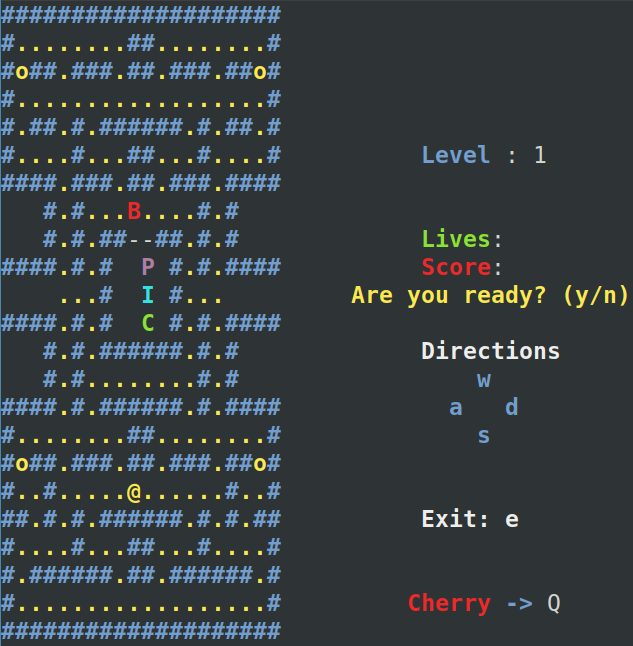
\includegraphics[width=.40\linewidth]{imagem.png}
\caption{Exemplo de aplicação do Ncurses}
\label{fig:xsort}
\end{figure}


% seção de metodologia %%%%%%%%%%%%%%%%%%%%%%%%%%%%%%%%%%%%%%%%%%%%%%%%%%%%%%
\section{Metodologia}

O método de pesquisa escolhido favorece a liberdade na análise dos conceitos e teorias que serão abordados, possibilitando assumir várias posições no decorrer do percurso. 

Para obter os resultados pretendidos, a equipe começará pela etapa de fundamentação e organização, onde serão levantados os principais conceitos sobre o tema e todo o planejamento estratégico da equipe durante o processo, a fim de aprimorar, embasar e organizar todo o trabalho. 

Em seguida, serão estruturados roteiros que irão guiar cada integrante na elaboracão das suas respectivas atividades semanais.

Ademais, serão feitas reuniões periódicas e ajustes das ações em andamento e também a elaboração de slides para auxiliar no processo de gravação das lições.

As aulas serão ministradas e gravadas com o suporte de toda a equipe e, posteriormente, organizadas para serem implementadas em uma plataforma de compartilhamento de vídeos escolhida  pelo  professor orientador. 

Por fim, um relatório final será elaborado e entregue ao departamento responsável, com o intuito de registrar e efetivar o trabalho desenvolvido pelos estudantes.
 
% subseção equipamentos %%%%%%%%%%%%%%%%%%%%%%%%%%%%%%%%%%%%%%%%%%%%%%%%%%%%%%
\subsection{Equipamentos Necessários}

%Listar os equipamentos necessários para a implementação do projeto.
\begin{enumerate}
 \item Programas de edição de vídeos, materiais de suporte e acesso à internet de qualidade. 
 \item Câmeras e computadores de qualidade para cada integrante da equipe.
 \end{enumerate}

% subseção com algoritmo %%%%%%%%%%%%%%%%%%%%%%%%%%%%%%%%%%%%%%%%%%%%%%%%%%%%%%
\subsection{Implementação}
A implementaçãao será feita por meio da criação de uma playlist em uma plataforma de compartilhamento de vídeos escolhida pelo professor orientador.

%\begin{algorithm}
%\caption{Algoritmo Ysort}\label{alg:ysort}
%\begin{algorithmic}[1]
%\Function{ysort}{estado}\Comment{retorna uma ação}
%\State \textbf{Entradas}: estado é a configuração atual do jogo
%\State $v\gets \mathrm{maxvalor}{(estado)}$
%\State \textbf{returna} a ação $a$ em sucessores(estado) cujo valor é $v$ %\Comment{comentario}

% \While{$r\not=0$}\Comment{We have the answer if r is 0}
% \State $a\gets b$
% \State $b\gets r$
% \State $r\gets a\bmod b$
% \EndWhile\label{euclidendwhile}

%\EndFunction
%\Function{maxvalor}{estado}\Comment{retorna o valor estático}
%\If{fim(estado)}
%   \State \textbf{retorna} estatico(estado)
%\EndIf
%\State $v \gets -\infty$
%\For{todas ações $a$ nos sucessores(estado)}
%    \State $v \gets \max{(v, \mathrm{minvalor}(a))}$
%\EndFor
%\State \textbf{retorna} $v$
%\EndFunction
%\Function{minvalor}{estado}\Comment{retorna o valor estático}
%\If{fim(estado)}
%   \State \textbf{retorna} estatico(estado)
%\EndIf
%\State $v \gets \infty$
%\For{todas ações $a$ nos sucessores(estado)}
%    \State $v \gets \min{(v, \mathrm{maxvalor}(a))}$
%\EndFor
%\State \textbf{retorna} $v$
%\EndFunction
%\end{algorithmic}
%\end{algorithm}

% seção Plano de Trabalho %%%%%%%%%%%%%%%%%%%%%%%%%%%%%%%%%%%%%%%%%%%%%%%%%%%%%%
\section{Plano de Trabalho}

 \begin{enumerate}
  \item Etapa de fundamentação e organização:
      \begin{enumerate}
         \item planejamento estratégico das ações e organização das tarefas;
         \item revisão bibliográfica;
         \item idealização dos códigos que serão utilizados;
         \item criação dos projetos de fixação(protótipos para treinamento e nivelamento).    
      \end{enumerate}    
  \item Criação do roteiro, slides e gravação do vídeo 1.
  \item Criação do roteiro, slides e gravação do vídeo 2.
  \item Criação do roteiro, slides e gravação do vídeo 3.
  \item Criação do roteiro, slides e gravação do vídeo 4.
  \item Criação do roteiro, slides e gravação do vídeo 5.
  \item Criação do roteiro, slides e gravação do vídeo 6.
  \item Entrega e validação do projeto pelo setor responsável.
\end{enumerate}

% seção Plano de Trabalho %%%%%%%%%%%%%%%%%%%%%%%%%%%%%%%%%%%%%%%%%%%%%%%%%%%%%%
\section{Cronograma}

%\begin{table}[ht] %modificação feita para fixar a tabela
%\begin{center}
% \caption{Tabela de cronograma do projeto de extensão}
%\begin{tabular}{|l|r|}
%  \hline \hline
%  \textbf{Etapas} & \textbf{Datas} \\ \hline \hline
%   Pesquisar o conteúdo & 24/06/2021 \\ \hline
%   implementação dos códigos & 05/07/2021 \\ \hline
%   roteiro dos vídeos & 12/07/2021 \\ \hline
%   Criação dos slides e vídeos  & 19/07/2021 \\ \hline
%   Editar os vídeos  & 23/07/2021 \\ \hline
%   Criação da Playlist  & 30/08/2021 \\ \hline
%   Elaboração do Relatório Final  & 01/09/2021 \\ \hline
%   Entrega e validação & 16/09/2021 \\ \hline \hline
%\end{tabular} 
%\label{tab:resultados}
%\end{center}
%\end{table}

 \begin{table}[ht] 
 \begin{center}
  \caption{Tabela de cronograma do projeto de extensão}
 \begin{tabular}{|l|l|l|l|l|l|l|l|l|l|l|l|l|}
   \hline \hline
        & \multicolumn{4}{|c|}{\textbf{mês 01}} & \multicolumn{4}{|c|}{\textbf{mês 02}} & \multicolumn{4}{|c|}{\textbf{mês 03}} \\ \hline \hline
     \textbf{ativividade semanal} & 01 & 02 & 03 & 04 & 05 & 06 & 07 & 08 &09 & 10&11&12& \hline
    Etapa de fundamentação e organização & X & X & X & & & & & & & & & & \hline
    Criação do roteiro e gravação do vídeo 1 & & & & X & & & & & & & & & \hline
    Criação do roteiro e gravação do vídeo 2 & & & & & X & & & & & & & & \hline
    Criação do roteiro e gravação do vídeo 3 & & & & & & X & & & & & & & \hline
    Criação do roteiro e gravação do vídeo 4 & & & & & & & X & & & & & & \hline
    Criação do roteiro e gravação do vídeo 5 & & & & & & & & X & & & & & \hline
    Criação do roteiro e gravação do vídeo 6 & & & & & & & & & X & & & & \hline
    Elaboração do relatório final & & & & & & & & & & X & X & & \hline
    Entrega e validação do projeto. & & & & & & & & & & & & X & \hline \hline
 \end{tabular}
 \label{tab:resultados}
 \end{center}
 \end{table}



% seção de impactos alcançados %%%%%%%%%%%%%%%%%%%%%%%%%%%%%%%%%%%%%%%%%%%%%%%%%%%%%%
\section{Impactos e Transferências}

% subseção de impacto científico %%%%%%%%%%%%%%%%%%%%%%%%%%%%%%%%%%%%%%%%%%%%%%%%%%%%%%
\subsection{Impacto Científico}

Não há impacto científico relevante.

% subseção de impacto tecnológico %%%%%%%%%%%%%%%%%%%%%%%%%%%%%%%%%%%%%%%%%%%%%%%%%%%%%%
\subsection{Impacto Tecnológico}

Não há impacto tecnológico relevante.

% subseção de econônimo %%%%%%%%%%%%%%%%%%%%%%%%%%%%%%%%%%%%%%%%%%%%%%%%%%%%%%
\subsection{Impacto Econômico}

Não há impacto econômico relevante.

% subseção de impacto social %%%%%%%%%%%%%%%%%%%%%%%%%%%%%%%%%%%%%%%%%%%%%%%%%%%%%%
\subsection{Impacto Social}

O projeto visa contribuir para a sociedade, ajudando a democratizar o conhecimento por intermédio de uma plataformar de compartilhamento de vídeos. 

% subseção de impacto ambiental %%%%%%%%%%%%%%%%%%%%%%%%%%%%%%%%%%%%%%%%%%%%%%%%%%%%%%
\subsection{Impacto Ambiental}

Não há impacto ambiental relevante.

% subseção de transferências %%%%%%%%%%%%%%%%%%%%%%%%%%%%%%%%%%%%%%%%%%%%%%%%%%%%%%
\subsection{Transferências}

O projeto transfere conhecimento de forma gratuita para toda a população, a fim de colaborar tanto no desenvolvimento intectual quanto cultural da sociedade.

% seção de resultados esperados %%%%%%%%%%%%%%%%%%%%%%%%%%%%%%%%%%%%%%%%%%%%%%%%%%%%%%
\section{Resultados Esperados}
Ao fim do curso, espera-se que os indivíduos contemplados tenham plena capacidade e autonomia na elaboração, manutenção e aperfeiçoamento de projetos e sistemas que utilizem a biblioteca Ncurses.

%%%%%%%%%%%%%%%%%%%%%%%%%%%%%%%%%%%%%%%%%%%%%%%%%%%%%%%%%%%%%%%%%%%%%%%%%%%%%%%%%%%%%%%%%%%%%%%%%%%%%%%%%%%%
% referências bibliográficas %%%%%%%%%%%%%%%%%%%%%%%%%%%%%%%%%%%%%%%%%%%%%%%%%%%%%%
%\section*{Referências Bibliográficas}

% cite todos, mesmo os não referenciados %%%%%%%%%%%%%%%%%%%%%%%%%%%%%%%%%%%%%%%%%%%%%%%%%%%%%%
\nocite{*}

% se necessario %%%%%%%%%%%%%%%%%%%%%%%%%%%%%%%%%%%%%%%%%%%%%%%%%%%%%%
% troca autor and autor por autor & autor, na bibliografia. O dcu usa "and"
%\renewcommand{\harvardand}{\&} % troca and pro &. O dcu usa "and"

% Estilos de bibliografia %%%%%%%%%%%%%%%%%%%%%%%%%%%%%%%%%%%%%%%%%%%%%%%%%%%%%%
% \bibliographystyle{abnt-alf} % Estilo alfabético da ABNT. Opção [num] para estilo numérico
%\bibliographystyle{apalike}
%\bibliographystyle{dcu} %citacao como (autor and autor, ano). Parece apalike. Rev. Control. Automacao. Use com harvard
%\bibliographystyle{agsm} % padrao harvard fica (autor & autor ano).
\bibliographystyle{acm}

% arquivo de banco de dados das referências %%%%%%%%%%%%%%%%%%%%%%%%%%%%%%%%%%%%%%%%%%%%%%%%%%%%%%
% renomear para o número do exercício correto
% o arquivo de bibliografia pode se chamar qualquer coisa, isso não muda o comando de gerar o PDF. 
% Por exemplo para 'mybiblio.bib', use \bibliography{mybiblio} e os comandos pdflatex e bibtex continuam os mesmos identicos com exN.
\bibliography{biblio}

\end{document}
